%--- 11 ----------------------------------------------------------------------------------
\item\vf{Le choix d’architecture peut avoir une influence sur la sécurité du système logiciel.}
{\vrai}
{L'architecture logicielle influence fortement les \textbf{propriétés} du système dont sa sécurité. Par exemple, il est plus difficle d'assurer la sécurité d'un système s'il est distribué (modèle en niveaux) que s'il est sur une unique machine.
\paragraph{}
Comme un choix d'architecture est quasi définitif, il y a des points de \textbf{non retour} lors du développement du système, la phase d'analyse du projet est donc primordiale.
\paragraph{Remarque:} il est \textit{impossible} d'optimiser toutes les propriétés d'un système (performance, sécurité, disponibilité, maintenabilité, fiabilité, tolérance aux pannes, comptabilité,...) car l'amélioration d'un critère se fait bien souvent au détrimant d'un autre. Des choix doivent donc être faits ( = COMPROMIS) quant aux critères les plus pertinents suivant l'application du système.

\paragraph{}
Afin d'améliorer la qualité d'un logiciel, une solution consiste à créer plus de tests unitaires pour couvrir le code au plus possible et effectuer soi-même d'avantage de "\textit{tests à la main}" pour évaluer tous les scénarios possibles d'utilisation. 
\paragraph{}Il est à noter que la \textit{qualité logicielle} est une notion très vague. Il faut se baser sur des critères (ex, norme ISO/CEI 9126: capacité fonctionnelle, fiabilité, facilités d'utilisation, performance, maintenabilité) et définir la façon de les mesurer pour avoir une évaluation qui a du sens.
}


%--- 12 ----------------------------------------------------------------------------------
\item\vf{Un design pattern est un template de code applicable automatiquement étant donné la spécifica-
tion d’une procédure/fonction/méthode.}
{\faux}
{Un design pattern est un \textbf{modèle de conception} général qui répond à une problématique récurrente en développement. Il s'agit d'une desciption de solution dont l'implémentation doit être adpatée aux cas particulier.
\paragraph{}Un pattern n'est donc pas automatiquement applicable.

\paragraph{Remarque:} les patterns sont regroupés selon 3 catégories:
\begin{enumerate}
\item \textbf{construction}: concerne l'instanciation des classes
\item \textbf{structuraux}: concerne l'organisation des classes entre elles
\item \textbf{comportementaux}: concerne la communication entre les objets
\end{enumerate}
}


%--- 13 ----------------------------------------------------------------------------------
\item\vf{Le design pattern du GoF Singleton permet de créer des instances d’une classe une à la fois.}
{\faux}
{Le pattern Singleton a pour objectif de garantir qu'une classe ne puisse être instanciée au plus que une seule fois.
\paragraph{}
Pour ce faire, on rend le constructeur privé (donc accessible uniquement depuis l'intérieur de la classe elle-même) et passe par une méthode pour instancier la classe. Cette méthode garantit qu'il n'existe que une seule instance au plus.
}


%--- 14 ----------------------------------------------------------------------------------
\item\vf{Le design pattern du GoF Builder est de type construction.}
{\vrai}
{L'objectif du pattern Builder est de déléguer la construction d'un objet à une autre classe afin de séparer la construction de l'implémentation.
\paragraph{}Il est utilisé, par exemple, dans le cas d'une classe ayant beaucoup de paramètres dans son constructeur ou plusieurs possibilités d'instanciation avec différentes règles.
\paragraph{}
Pour ce faire, le pattern utilise une classe abstraite qui définit un comportement commun à la création des objets et des classes concrètes, qui étendent celle-ci, pour définir les différents cas possibles de création. Une autre classe, quant à elle, passe par un de ces \textit{builders} concrets pour instancier la classe abstraite.
}


%--- 15 ----------------------------------------------------------------------------------
\item\vf{Pour appliquer le design pattern du GoF Facade, il faut impérativement rendre toutes les
procédures/fonctions/méthodes des sous-systèmes à cacher privées.}
{\faux}
{Le pattern façade est un \textbf{point d'entrée} pour un sous-système, il facilite l'accès à toutes ses fonctionnalités. La façade délègue les requêtes du client aux objets appropriés. Cependant, il s'agit d'une \textit{alternative simplifiée} pour utiliser le système, elle ne bloque pas l'accès individuel aux différentes classes (\textbf{pas d'encapsulation} !)
\paragraph{}
L'intérêt du pattern est de diminuer le couplage entre le client et les classes du sous-système. La façade fait le lien avec les différentes interfaces du sous-système de sorte que l'implémentation des classes ou du client peut changer sans impacter le fonctionnement.
\paragraph{}
Le client peut donc au choix utiliser une des façades du système pour accéder à ses fonctionnalités ou instancier directement une partie du système.
}


%--- 16 ----------------------------------------------------------------------------------
\item\vf{Le design pattern du GoF Template permet d’implémenter un algorithme incomplet avec des
« trous » à remplir (hooks).}
{\vrai}
{Le pattern Template ou Strategy permet de définir une \textbf{famille d'algorithmes} et de choisir dynamiquement (lors de l'exécution) celui à utiliser.
\paragraph{}
Pour cela, le pattern utilise une classe abstraite (la \textit{Stratégie}) qui définit une méthode avec les parties communes d'un algorithme et des trous, représentant les parties variables, qui devront être remplis par des classes concrètes qui étendent cette \textit{Stratégie}. Pour choisir l'algorithme a utiliser, le client possède une variable du type de la classe abstraite et il instancie une des classes conrètes au choix.
}


%--- 17 ----------------------------------------------------------------------------------
\item\vf{La programmation impérative met l’accent sur le comment un programme fonctionne.}
{\vrai}
{Un programme, en prog. impérative, possède à tout instant un \textbf{état} qui est définit par la valeur en mémoire de ses variables (à l'image des objets en POO). Il est constitué d'une \textbf{séquence d'instructions} exécutées de façon "linéaire" et qui modifient l'état du programme. 
\paragraph{}
Il s'agit de l'opposé de la programmation déclarative.
\paragraph{}
\textit{Exemples: Fortran, Algol, Pascal, Basic, C,...}
}


%--- 18 ----------------------------------------------------------------------------------
\item\vf{La programmation déclarative met l’accent sur le comment un programme fonctionne.}
{\faux}
{La programmation déclarative se concentre sur \textbf{ce que} le programme doit faire et ne se soucie pas de comment il va y parvenir, on fournit donc seulement une "description" des résultats que l'on attend.
\paragraph{}
Ce paradigme est également marqué par l'\textbf{absence d'effets de bord},c'est-à-dire qu'une fonction ne modifie pas un état autre que celui de ses valeurs de retour.
\paragraph{}
Il s'agit de l'opposé de la programmation impérative.
\paragraph{}
\textit{Exemples: XML, SQL, Prolog, ...}

}


%--- 19 ----------------------------------------------------------------------------------
\item\vf{La programmation fonctionnelle est plus proche de l’impérative que de la déclarative.}
{\faux}
{En programmation fonctionnelle, l'exécution d'un programme est une séquence d'évaluations de \textbf{fonctions mathématiques}. Le résultat d'une telle fonction ne dépend \textbf{que de ses entrées} et retourne toujours une même valeur de sortie pour une entrée donnée.
\paragraph{}
Les variables n'ont \textbf{pas d'état} et les données ne sont pas mutables, les seules valeurs fournies sont passées en paramètres aux fonctions.
\begin{figure}[h!]
\center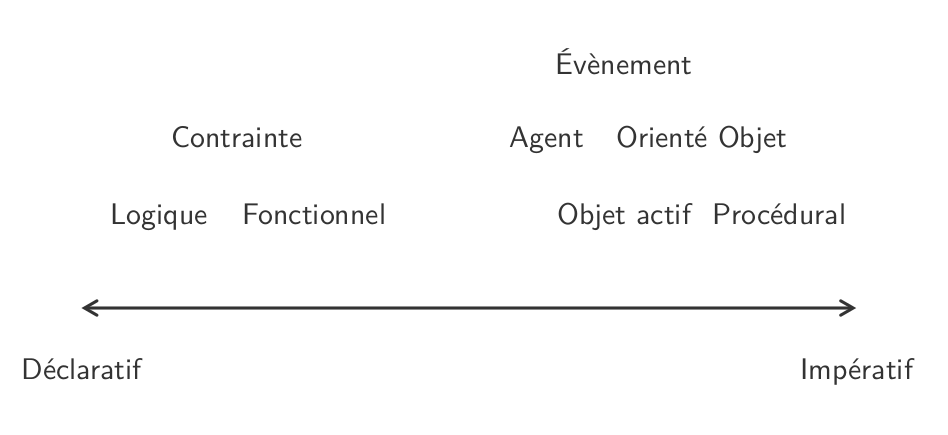
\includegraphics[scale=.3]{images/vue-paradigmes}
\caption{Vue générale des paradigmes}
\end{figure}
\paragraph{Remarque: }
Le point d'entrée du programme est une fonction main qui produira un résultat en appelant d'autres fonctions.
}


%--- 20 ----------------------------------------------------------------------------------
\item\vf{La programmation fonctionnelle est plus éloignée de l’impérative que de la déclarative.}
{\vrai}
{}